\documentclass{elsarticle}
\usepackage{amssymb}
\usepackage{amsmath}
\usepackage{bigdelim}
\usepackage{multirow}
\usepackage{hyperref}
\usepackage{graphics}
\usepackage{algorithm}
\usepackage{algorithmic}
\usepackage{subfigure}
\usepackage{kbordermatrix}
\usepackage{booktabs}

%\usepackage{algorithmicx}
\journal{Physica A}

\newtheorem{definition}{Definition}


\begin{document}

\begin{frontmatter}
\title{A Complex Network Model of Knowledge Collaboration in Virtual Community: Based on Wiki Community
}
\author[buaa]{Jun Wang}
\ead{king.wang@buaa.edu.cn}

\author[buaa]{Yunpeng Wu}
\ead{yunpeng.wu@sem.buaa.edu.cn}

\author[buaa]{Xin Jin}
\ead{sss}

\address[buaa]{School of Economics and Management, Beihang University, 
Beijing 100083, P.R. China}

\begin{abstract}
  Wikipedia is a typical konwledge collaboration community. Though
  it's network topology has been studied by many schloars, the
  relationship among users and the affiliation among topic and users 
  still remain ignored. This paper propose two kinds of networks:
one-dimensional network aiming at modelling users collaboration in
this commutity and
two-dimensional network aiming at modelling users and topics
affiliation. The result shows the two kinds of networks are both
complex networks.  The one-dimensional network has scale-free
structure, and its degree distribution is subject to the power law and
possesses obvious “small world” phenomenon. At the early stage of the
network development, the network does not possess hierarchical
topology. However, when the network size increases with time, the
network gradually reveals unapparent hierarchy. Furthermore, we
observed that there is positive relationship between the density of
the one-dimensional network and the scale ratio, and  an
insignificant positive correlation between the clustering coefficient
and the scale ratio. In the two-dimensional network model, we found
the theme degree and the topic size have consistent law: subject to
the power-law distribution. In addition, the cumulative distribution function of the topic size is exponential function.


\end{abstract}

\begin{keyword}
Wikipedia, Knowledge collaboration network, Scale-free structure,
Small-world effect, Topic approximation, Scale ratio
  
\end{keyword}
\end{frontmatter}

\section{Introduction}
\label{sec:introduction}

Research of complex network is being popular in recent years among scholars
especially from areas of computer science and social science.
 The scientific understanding to the quantitative and
qualitative characteristics of complex network has been studied in
different aspects such as sociology, mathematics, life sciences,
engineering and many others. The main differences between complex
network and ordinary network are  some non-trivial
topologicl features occured in complex network such as “small worlds” effect\cite{Watts2003}, scale-free\cite{PhysRevLett.90.058701},
power law\cite{wang2003cns} and so on. A typical example of complex network is collaboration system. In this network, collaborators are represented by nodes of the network
and their connnections are represented by edges. A piles of literatures
have analyzed the statistical propeties\cite{albert-2002-74,dorogovtsev2002en,pastorsatorras2004eas} and give the mechanism of
the network evlovement.


%In recent years, bipartite networks have attracted more and more people's attention [10-13]. Factuallyt, many real-world networks are naturally bipartite, such as the actors-films network [11], the Scientist Co-authorship Collaboration network [12-13], the knowledge-cooperation network and so on.

Wikipedia is the world largest online-encyclopedia based on wiki
system,  characterized as "ultra-lightweight" content management systems
\cite{mattison2003qst}. It is often seen as the typical
knowledge-cooperation social newtork in a  virtual
practice community. The huge content serves as an excellent example of
a large complex network\cite{Barabasi2003}, thus attracted the intense attention of scholars
because of its' unique characteristics. Unlike other social networks on the
Internet,such as blog,  the
collaboration in Wikipedia is expanding denotedly and connotedly while the collaboration in blog is non-themed or variable- themed. It will talk about a topic with a very full depth\cite{Sauer2005}.

Topics and users constitute  Wikipedia. A topic is a content entry
of Wikipedia relatively indepentent, meanwhile
cross-referred to other topics. The topology of topic netwotk  has
been examined
 from several facets. Capossi etc described topics by vertices and hyperlinks between them as edges, thus represent
this encyclopedia as a directed graph\cite{capocci-2006}. Their research shows Wikipedia has
similar topological properties  to the World Wide Web. Zlati\'{c} etc use
same methods and thoroughly studied the network characteristics such as as their degree distributions, growth, topology, reciprocity, clustering, assortativity, path lengths, and triad
significance profiles in different language versions\cite{zlatic:016115}. Bolikowski
focused on  the link between diferent language edition of topics and found
the topic size distribution obeys the power
law\cite{bolikowski-2009}. Some other scholars analyzed
the network alongwith time slices\cite{buriol2006taw}. The interesting thing is
, as metioned before, though users are another foundation of Wikipedia
content creation, they are ignored by current researchers in network
analysis. There are interaction between users themself and connections
between users and topics, both form a network and remain unclear of the topology and
properties of the network.    



 This paper keeps eyes  on these two kinds of networks: the
 one-dimensional network, representing users connections; the
 bipartite network, which ties users and topics. Through an
 empirical study of en-Wikipedia network’s data  from January
 2004 to January 2008, we discover that many properties of these two
 networks are similar to other complex networks. 

The rest of the paper is organized as follows. In section 2, we
introduce the complex social network to model  knowledge
collaboration in Wikipedia community. The empirical analysis of the one-dimensional
properties is presented in section 3. Section 4 examines properties
and scale of the  bipartite network. Section 5 is
the conclusions and discussions.

\section{The network structure of knowledge collaboration in Wikipedia
community}
\label{sec:netw-struct-wiki}

 Wikipedia
can be depicted as an open content encyclopedia. Allowing unrestricted access to any third party to copy, modify,
thus, it  provides great convenience for people from various
sectors. On the meantime, the users can increase their knowledge and
enrich themselves. As of April 25, 2009, according to Wikipedia
statistics\footnote{http://s23.org/wikistats/wikipedias\_html.php}, the English version has
16,550,111 entries and more than  9,505,160 registered users. Wikipedia allows users to edit the topics collabortively. They can add
new content, fix other's error, revert previous edit. The
collaboration content creation activities thus connect the user who
engaged in the same topic into a network, which is our reseach object. 


As to the characteristics of Wikipedia knowledge collaboration
network, we build a collaborative 
knowledge network model, shown in Figure \ref{fig:two-layer}. There are also two
types of ties: connections, noted as $C$, and afilliations, noted as $A$. $C$
is the collaboration among users, shown by white lines, while
$A$ express the affiliation between topics and users, noted as $T$ and $U$ respectively, shown as dark color lines. 

\begin{figure}[h]
  
  \centering
  \scalebox{0.8}{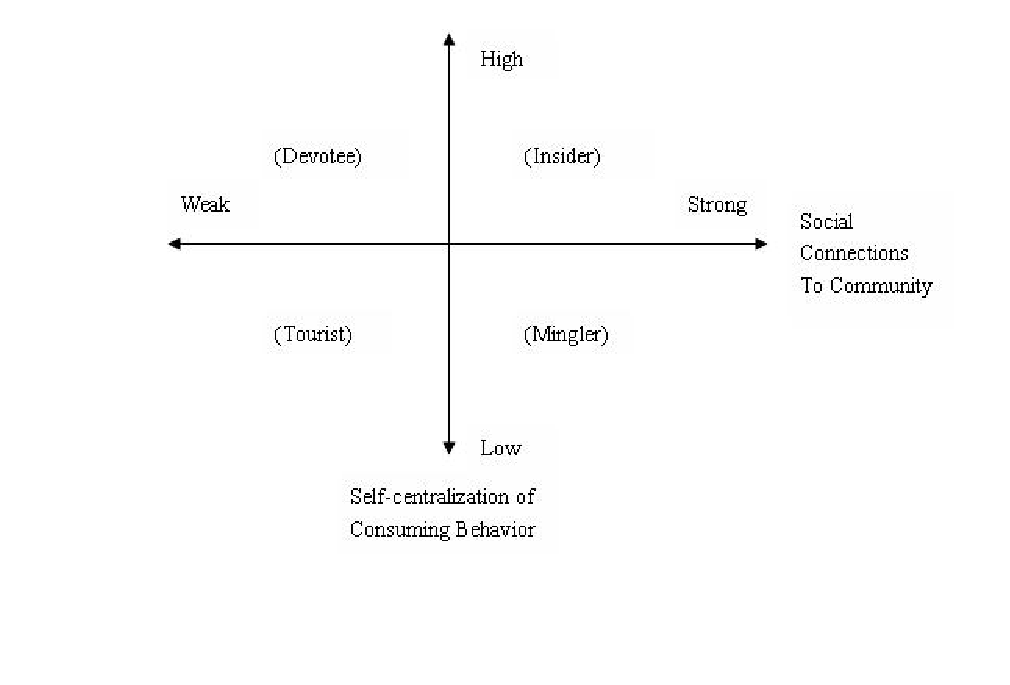
\includegraphics{01}}
  \caption{The Two-dimensional, Wiki-based Knowledge Collaboration Network Model}
  \label{fig:two-layer}
\end{figure}

This figure depicts  two kind of  networks: one-dimensional networks of
single-layer and bipartite two-dimensional networks. 
In the single-layer networks, all the users involved in the same topic
collaboration process builds an Undirected and Unweighted Complete
Sub-graph (UUCSG), shown as [u1-u2] [u3-u6] [u6-u10] [u9-u12] in
Figure \ref{fig:two-layer}. The entire single-layer network is composed of $N$ UUCSGs, in
which $N$ represents the number of topics. The whole network can be
expressed as an adjacency matrix, noted by $B_u$.
For bipartite networks, it's UUCSG is constructed by all the UUCSGs in
 the single-layer networks and the topics which the UUCSGs belong
 to. The number of nodes is equal to the numbers of the user
 nodes. Each bipartite network focuses on  certain areas but ignore
 others. It  constitutes a circle which has high
 cohesion but loosely-coupled. Therefore, the bipartite networks can be described as an
 adjacency matrix $B_t$. 
\begin{displaymath}
\scalebox{0.73}{
$
  B_u = \bordermatrix{%
    &u_1&u_2&u_3&u_4&u_5&u_6&u_7&u_8&u_9&u_{10}&u_{11}&u_{12} \cr
  u_1&0&1 \cr
  u_2&1&0 \cr
  u_3&&&0&1&1&1 \cr
   u_4&&&1&0&1&1 \cr
 u_5&&&1&1&0&1 \cr
 u_6&&&1&1&1&0&1&1&1&1 \cr
 u_7&&&&&&1&0&1&1&1 \cr
 u_8&&&&&&1&1&0&1&1 \cr
u_9&&&&&&1&1&1&0&1&1&1 \cr
  u_{10}&&&&&&1&1&1&1&0&1&1 \cr
   u_{11}&&&&&&&&&1&1&0&1 \cr
  u_{12}&&&&&&&&&1&1&1&0 \cr
}
$

$
   B_t = \bordermatrix{%
    &T_1&T_2&T_3&T_4 \cr
   u_1&1 \cr
   u_2&1 \cr
    u_3&&1 \cr
    u_4&&1 \cr
    u_5&&1 \cr
    u_6&&1&1 \cr
    u_7&&&1 \cr
    u_8&&&1 \cr
    u_9&&&1&1 \cr
    u_{10}&&&1&1 \cr
    u_{11}&&&&1 \cr
    u_{12}&&&&1 \cr
}
$
}
\end{displaymath}

We define scale ratio  between users and topics  in
 the bipartite networks,
 described as
 \begin{math}
 W = N_{user}/N_{topic}   
 \end{math}.
We then can depict the whole collaboration activities in the
content-generating community and analyze their properties.
\section{The empirical study of single-dimensional  knowledge collaboration network}
\label{sec:empir-study-single}
Wikimedia provides the archivess of  wikipedia contents dumped
regularly from
Wikipedia's website.  There are several types of archive: 
pages\nobreakdash{-}articles contains current versions of article content,
pages-meta-current is  a   complete current snapshot archive. Besides pages-articles
content, discussion and user pages are also included.  The third type
is pages-meta-history contains complete text of every revision of
every page which very suitabel  for research.
In this study, we choose
“enwiki-20081008-stub-meta-history.xml”\footnote{http://download.wikimedia.org/enwiki/20081008/} as our research
data. It contains no page text but only revision metadata before
December 8th 2008. Since our concern is on the collaboration activies,
the text content of the topics is not neccesary to our study. Because
the Wikipedia community was in its early stage
 before 2003, we re-select the data from 2004 to 2008 in order to
better observe the changes of the network  properties at different time periods. We divided the time duration into months, build 48 sub-networks of each month from January 2004 to December 2007 and analyze the properties of the 48 sub-networks.

Before analysing, The data archive has to be cleansed and refined:
\begin{enumerate}
\item Abandon all the contributors data in the above-mentioned time
  periods and all the related contributors versions, discussion pages, 
  for these data are useless to our study.
\item Exclude anonymouse contribution. Wikipedia allows anonymous edit
  and show the editor's IP addresses. However, we are unable to check
  the identity and track his activities without user ID. Only
  registered user are included in this study.
\item Delete isolated nodes, namely, the topics which have only one
  contributor. We presume that there is no collaboration relationship
  between this user and other users under isolated nodes.

\end{enumerate}
 
In order to illustrate the data changes, ultimately the 24
odd-numbered subnets are selected as representatives to describe the
network characteristics. The summary of the cleared network data are
shown in table \ref{tab:wikidata-summary}, which clearly describes the static parameters
changes of the knowledge collaboration networks over time. The
increasing amount of the one-dimensional knowledge collaboration networks is decided by
the growth of the Wikipedia community. With the Wikipedia culture is
receiving increasing attention since 2004, the scale of the Wikipedia
virtual community is gradually expanding. There were more than 1400
million pages in Wikipedia until October 2008. The network scale grew
quickly from 2004 to the mid of 2007, nevertheless, declined gradually
later.
% Table generated by Excel2LaTeX from sheet 'Working'
\begin{table}[htbp]
  \label{tab:wikidata-summary}
  \caption{The 24 odd-numbered Wikipedia data summary from 2004 to 2007}
   \begin{tabular}{lllllll}
     \toprule
        & Users & Pages & W &  \parbox{1.4
cm}{Average Degree} &  \parbox{1.7cm}{Clustering Coefficient} &  Density \\\hline
      {\bf Jan-04} & 2634  & 18650 & 0.141233 & 83.125 & 0.642991 & 0.063141 \\
    {\bf Mar-04} & 4807  & 37733 & 0.127395 & 85.467 & 0.640963 & 0.035567 \\
    {\bf May-04} & 5344  & 35688 & 0.149742 & 88.263 & 0.629839 & 0.033039 \\
    {\bf Jul-04} & 6814  & 57986 & 0.117511 & 94.662 & 0.651261 & 0.027789 \\
    {\bf Sep-04} & 8621  & 66186 & 0.130254 & 113.226 & 0.648146 & 0.026271 \\
    {\bf Nov-04} & 11757 & 97336 & 0.120788 & 116.668 & 0.654176 & 0.019848 \\
    {\bf Jan-05} & 12343 & 61389 & 0.201062 & 91.989 & 0.632225 & 0.014907 \\
    {\bf Mar-05} & 15943 & 91034 & 0.175132 & 102.796 & 0.630041 & 0.012896 \\
    {\bf May-05} & 20323 & 113260 & 0.179437 & 104.417 & 0.678814 & 0.010276 \\
    {\bf Jul-05} & 27127 & 140591 & 0.19295 & 135.279 & 0.647197 & 0.009974 \\
    {\bf Sep-05} & 30125 & 153697 & 0.196003 & 125.932 & 0.650241 & 0.008361 \\
    {\bf Nov-05} & 37182 & 190484 & 0.195197 & 117.661 & 0.662213 & 0.006329 \\
    {\bf Jan-06} & 61349 & 276782 & 0.221651 & 156.882 & 0.676517 & 0.005114 \\
    {\bf Mar-06} & 83577 & 331995 & 0.251742 & 157.1 & 0.7016 & 0.003759 \\
    {\bf May-06} & 95454 & 336581 & 0.283599 & 157.751 & 0.705743 & 0.003305 \\
    {\bf Jul-06} & 104253 & 371719 & 0.280462 & 152.648 & 0.712564 & 0.002928 \\
    {\bf Sep-06} & 122794 & 395049 & 0.310832 & 151.984 & 0.697645 & 0.002475 \\
    {\bf Nov-06} & 138858 & 396855 & 0.349896 & 154.183 & 0.724345 & 0.002221 \\
    {\bf Jan-07} & 154494 & 449403 & 0.343776 & 151.459 & 0.720432 & 0.001961 \\
    {\bf Mar-07} & 168900 & 492561 & 0.342902 & 176.884 & 0.719482 & 0.002095 \\
    {\bf May-07} & 160008 & 474705 & 0.337068 & 224.048 & 0.693921 & 0.0028 \\
    {\bf Jul-07} & 138543 & 432391 & 0.320411 & 174.423 & 0.701221 & 0.002518 \\
    {\bf Sep-07} & 146961 & 454726 & 0.323186 & 230.81 & 0.702132 & 0.003141 \\
    {\bf Nov-07} & 145782 & 440376 & 0.33104 & 189.126 & 0.71322 & 0.002595 \\\bottomrule
       \end{tabular}
  \label{tab:addlabel}
\end{table}
In order to observe the network changes with time in more details,
this paper gives a more figurative description of the topological
properties of the one-dimensional complex network of
knowledge-oriented collaboration. We will discuss from five aspects: Power Law, average degree, clustering coefficient, small world and hierarchical network.

\subsection{The analysis of scale-free structure}
\label{sec:analysis-scale-free}

Degree distribution is one of the most
importand peoperty of a network because of its inherent important
topology information and network evolution information.   The degree of
the node refers to the number of the node's adjacent nodes or the
number of adjacent edges.  Barabási and
Albert proposed a scale-free network model, known as the BA
model\cite{barabasi1999esr}. In this model,  the degree distribution of nodes   applies to power-law distribution.  In our network descriptions, the degree of Node $i$ is described as follow: 
\begin{equation}
  K_i=\sum_{j\in\mu_i}C_{ij}
\end{equation}

$\mu_j$represents the adjacency matrix of the user node. If node $i$
and $j$ are linked, the value  is 1, otherwise 0. Degree distribution
of a node
refers to the probability of a node with exact degree $k$ in the
selected network. Studies show that degree distribution of BA
scale-free network is in line with the shifted power-law, that is
$P(K=k)\thicksim k^\gamma+\alpha$, both the $\gamma$ and $\alpha$ are 
constants. 


The degree distributions of the above 24 Wikipedia subnet are
displayed as curves in double logarithmic coordinates, as shown in
Figure \ref{fig:degree-distr}. To show conveniently, each subgraph in Figure \ref{fig:degree-distr} identifies
the subnets of three months.
\begin{figure}[htpb]
 
  \centering
  \subfigure[ ]{
     \scalebox{0.18}{\includegraphics{02-1}}
   } \quad
  \subfigure[ ]{ 
       \scalebox{0.18}{\includegraphics{02-2}}
   } 
   
    \subfigure[ ]{
     \scalebox{0.18}{\includegraphics{02-3}}
   } \quad
  \subfigure[ ]{ 
       \scalebox{0.18}{\includegraphics{02-4}}
   } 
  
    \subfigure[ ]{
     \scalebox{0.18}{\includegraphics{02-5}}
   } \quad
  \subfigure[ ]{ 
       \scalebox{0.18}{\includegraphics{02-6}}
   } 

    \subfigure[ ]{
     \scalebox{0.18}{\includegraphics{02-7}}
   } \quad
  \subfigure[ ]{ 
       \scalebox{0.18}{\includegraphics{02-8}}
   } 
   \caption{Distribution of degree in odd months under Log-Log
     coordinates from 2004 to 2007}
    \label{fig:degree-distr}
\end{figure}

Master equation method is adopted to further analyze degree
distributions of the above collaboration networks\cite{PhysRevLett.85.4633}. Degree
distribution function of the BA network can be similarly described by
the Power-law function with Power index for the 3. As Figure \ref{fig:degree-distr} shows,
the slope of the power-law distribution functions of the 
collaborative knowledge network in log-log coordinates is approximate
to 0.01--0.001, and the functions have similar interception of 
linear approximatiton. Therefore, these networks are  BA scale-free network and the properties  conform to the
BA scale-free network.

The size of these networks are continually growing. Every day there
are many new users joining in Wikipedia
community.  
The new node prefers to connect to those
“big nodes” with higher degree. This phenomenon is also known as "the
rich get richer" or "Matthew Effect". In our case, new users tend to participate in editing
the topics whose editors are “big nodes”. Here
the so-called “big” nodes are referred to as “more active users.” The way of network evolution
is moving closer to the central node, thereby forms the polarization
between the rich and the poor. The scale-free networks can grow from
very few nodes to a complex network with a large number of nodes.  When the
quantity of the network nodes grows to a certain scale, the network
will indicate that: only a few users have a large number of connected
nodes, while the rest of  users only have a small number of
connections, namely, the “long tail” phenomenon. 


\subsection{The changes of average degree}
\label{sec:chang-aver-degr}

With the development of the Wikipedia culture, more and more people devote
their efforts to contribute to the free encyclopdia.  There are two
reasons explain the increase of the users: the first
is the increasing new topics. According to the internal data of
Wikipedia, new topics have increased dramatically each year.
Wider scope of content enables more users to join in the topic editing. The
second is that more and more users are participating in the
contribution under the existing topics. Therefore, the average degree
is introduced to describe the number of relationship within Wikipedia users
network, noted as $AverageDegree = \sum_iK_i/\text{Number of Users}$

The change curve of average degree over time is shown in Figure \ref{fig:average-degree}. 
\begin{figure}[htpb]
  \centering
  \scalebox{0.3}{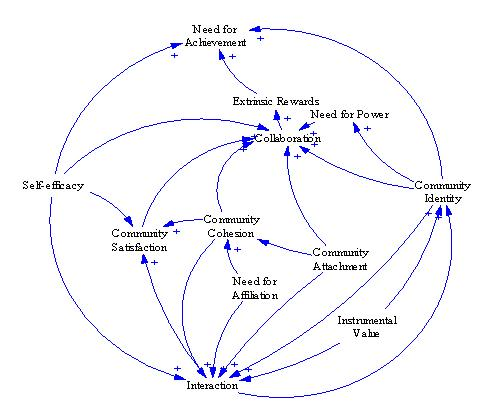
\includegraphics{03}}
  \caption{The changes of the average degree from 2004 to 2007}
  \label{fig:average-degree}
\end{figure}
Obviously, the average degree presents an upward trend. The upward shock  indicates the number of the “innate
relations” of the  networks increasing intensively. In the Wikipedia
community, average degree concussion is often caused by the editing shock of
the topic node. Take the topic “the Festival” as example, the number
of the editing increases apparently in January and February of each
year. Another example is "financial crisis". The amount of editing  increases sharply in 2008. Therefore, the average degree is closely related to the degree of concern within Wikipedia topic.

\subsection{ The changes of clustering coefficient}
\label{sec:chang-clust-coeff}

Clustering coefficient, also known as congregate extent, describes the
clustering effect of the complex network, reflecting the property
of "Like attract like". Suppose that the degree of a node $i$ in the
network is $k_i$  , $k_i$ -nodes are neighbor's of $i$ which
connecting to $i$.  $C_i$  refers to the Clustering
Coefficient of the Node $i$,  defined as the ratio between the
real number of the edges among the $k_i$-nodes, noted as $E_i$, and the possible total
number of edges: $k_i(k_i-1)/2$. So  $C_i=2E_i/k_i(k_i-1)$. The
Clustering Coefficient of the whole network $C$ is the average of all
the nodes’ clustering coefficient.In one-dimensional network, $C$ value  tend to be a certain non-zero
constant despite of the increasing of network size, that is, when
$N\rightarrow\infty,C=O(1)$ . The clustering coefficient of the
free-scale network  can be defined as $C=\beta[\ln(t)]^2/t$. $\beta$
is network evolution constant.

The changes of the Clustering Coefficient of the knowledge
collaboration one-dimensional network are shown in Figure \ref{fig:cluster-coeff}.
\begin{figure}[htpb]

  \centering
  \scalebox{0.3}{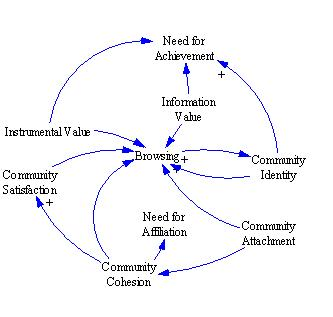
\includegraphics{04}}
  \caption{ The changes of clustering coefficient from 2004 to 2007}
    \label{fig:cluster-coeff}
\end{figure}
 
 Figure \ref{fig:cluster-coeff} 
shows that the clustering coefficient averages to 0.55. In fact, many
types of complex networks, especially social networks, aren’t entirely
random network. As a community of practice, Wikipedia network shows
the "people to group" features. This conclusion is obvious, according
to the definition of communities of practice: the people who pay
attention to certain subject, and with strong passion for this topic,
increase their knowledge and skills through communicating and
exchanging knowledge in this field with each other sustained[18].
Members of the community participate in editing the pages of some topics  in accordance with their interests, hobbies, professional. 



\subsection{“Small world” phenomenon }
\label{sec:small-world-phen}

Small world phenomenon reflects a kind of social network
characteristics: most of the people and their friends are in the same
circle of people. Many studies have shown that small-world phenomenon
exists in many real networks. Small world phenomenor indicated by two
characteristics: shorter average path length and higher clustering
coefficient. The average path length $L$ is the average length of
all minimum number of edges connecting a pair of vertices. Because of
the large calculation scale of the average path and the limitation of
calculation, this study only calculates and analyzes the average
distances of the 6 sub-networks: the 1st, 18th, and 35th weeks of
2004 and 2005 whose size are still relatively small, as shown in table
2.

\begin{table}[htpb]
  \centering
 \caption{The clustering coefficient and average distance} 
 \begin{tabular}{lcc}
   \toprule
    &Clustering Coefficient&Average distance\\\hline
  04 1st week&0.5085&2.546\\
  04 18th week&0.5020&2.745\\
  04 35th week&0.4965&2.819\\
  05 1st week&0.4804&2.980\\
  05 18th week&0.4956&3.009\\
  05 35th week&0.4991&3.191\\\bottomrule
   \end{tabular}
 \label{tab:small-world}
\end{table}

Table \ref{tab:small-world} indicate two conclusions. On the one hand, the
clustering coefficients discussed above are around 0.5, which is higher. On the other
hand, the average path length is small, that is, any two people
in the network can find each other through less than 4 individuals on
average. Because of the shorter path between nodes, the cost of
information transferring is lower than in
networks with other structures. The result shows a user is easy to find an cooperator
alongwith an proper path, which in turn improve the efficiency of collaboration.



 \subsection{Hierarchical network}
\label{sec:hierarchical-network}

Studies have shown that the topology modules in some networks are
organized in accordance with Hierarchy\cite{PhysRevE.67.026112,PhysRevE.65.066122}. One of the most
important quantitative indicators of the hierarchical Network is the
dependent relationship between clustering coefficient and degree of a
node obey
the power-law distribution: $C_i\sim k_i^{-\beta}$. This indicates the
nodes with very small degree possess high clustering coefficient,
while the nodes with high degree have lower clustering coefficient, whose role is to connect the different modules.

To test whether the on-domensional networks are hierarchy networks, we select subnet of  January and
March of 2004, 2005, and 2006  as representatives, shown in
Figure \ref{fig:hierarchy}. These figures show the  network doesn’t show obvious
linear features when the network scale is small. The small scale network is consistent with the
BA scale-free network characteristics and doesn’t possess hierarchical
topology. Furthermore, the clustering coefficient $C_i$
shows little direct relation with the degree $k_i$ of the node $i$. We see the  network doesn’t contain the
hierarchical mechanism which is conductive to the module emergence at
the early stage of the structuring process. However, when the network
size increases with time, the network gradually reveals certain level
of hierarchy. As the
network size increases, network mechanism helps the emergence of
modules. 


\begin{figure}[htpb]
  \centering
  \subfigure[ ]{
     \scalebox{0.18}{\includegraphics{05-1}}
   } \quad
  \subfigure[ ]{ 
       \scalebox{0.18}{\includegraphics{05-2}}
   } 
  
    \subfigure[ ]{
     \scalebox{0.18}{\includegraphics{05-3}}
   } \quad
  \subfigure[ ]{ 
       \scalebox{0.18}{\includegraphics{05-4}}
   } 
   
    \subfigure[ ]{
     \scalebox{0.18}{\includegraphics{05-5}}
   } \quad
  \subfigure[ ]{ 
       \scalebox{0.18}{\includegraphics{05-6}}
   } 
   \caption{Relationship between cluster coefficient and degree under
     Log-Log coordinate}
   \label{fig:hierarchy}
\end{figure}

\section{The  study of the wiki bipartite network}
\label{sec:4the-pilot-study}

In recent years, bipartite networks have attracted more and more people's attention\cite{watts1998sw,morris-2005,PhysRevE.64.026118}. Actually, many real-world networks are naturally bipartite, such as the actors-films network\cite{watts1998sw}, the Scientist Co-authorship Collaboration network\cite{morris-2005,PhysRevE.64.026118}, the knowledge-cooperation network and so on.

The two-dimensional networks are  bipartite network much larger than the one-dimensional
networks, interacting more and collaborating more among users. Not only
direct collaboration, but indirect collaboration and topic nodes are
also included in this network model. Therefore, it is  significant to study the
two-dimensional networks of the knowledge collaboration. 

\subsection{The theme distribution of the user node}
\label{sec:theme-distr-user}

Topics are created and edited by users. The affiliations depicted in
figure \ref{fig:two-layer} demonstrate these kind of relationships. 
The theme degree $K_t$ is the quantification of
affiliations between  the user nodes and topic nodes. For a given user
node $i$ the theme degree is a random variable, 
defined as:
\begin{equation}
  \label{eq:1}
  K_{ti}=\sum_{j \in t_i} T_{ij}
\end{equation}
In this definition, $t_i$ denotes the adjacency matrix of  $Bt$
matrix of the user node $i$. If the user node $i$ get involved in  edting the topic
$j$, then $T_{ij}=1$, otherwise
it is 0. The theme degree is
another important quantified indicator that portrays the degree of
user participating in the topic.  Figure \ref{fig:theme-degree} presents the curves of the theme degree
probability  distribution  in odd months of 2004-2007 under Log-Log
coordinates. 

\begin{figure}[htpb]
  \centering
  \subfigure[ ]{
     \scalebox{0.18}{\includegraphics{06-1}}
   } \quad
  \subfigure[ ]{ 
       \scalebox{0.18}{\includegraphics{06-2}}
   } 
  
    \subfigure[ ]{
     \scalebox{0.18}{\includegraphics{06-3}}
   } \quad
  \subfigure[ ]{ 
       \scalebox{0.18}{\includegraphics{06-4}}
   } 
  
    \subfigure[ ]{
     \scalebox{0.18}{\includegraphics{06-5}}
   } \quad
  \subfigure[ ]{ 
       \scalebox{0.18}{\includegraphics{06-6}}
   } 

    \subfigure[ ]{
     \scalebox{0.18}{\includegraphics{06-7}}
   } \quad
  \subfigure[ ]{ 
       \scalebox{0.18}{\includegraphics{06-8}}
   } 
   \caption{Distribution of theme degree in odd months from 2004 to
     2007}
   \label{fig:theme-degree}
\end{figure}

Obviously, the theme distribution curve of the bipartite network is
similar to the one-dimentional network, which subjects to the power-law distribution, that is: 
\begin{equation}
  \label{eq:2}
  P(k_t)\sim k_t^{\gamma}+\alpha
\end{equation}


As network size expanding,  new nodes prefer to connect with those
“big” nodes with higher degrees. This result means in a enough large
network a small number of user nodes connect with a great part of
themes nodes, while most of user nodes only participate in a small number of topic contribution, presenting obvious feature of “the Long Tail”. 
\subsection{The study of topic size}
\label{sec:topic-size}

In the the bipartite network, besides the number of topic
nodes, another important quantitative indicator is the number of user
nodes of the topic nodes, which portrays the number of user nodes
belonging to a certain  topic node $j$, noted as topic node size: $s_j
= \sum_{i \in t_j}T_{ij}$. $t_i$  represents
the adjacency matrix of the $Bt$ matrix of the topic node $j$. If the user
node $i$ belongs to the topic node $j$, then $T_{ij}=1$ , otherwise 0. It is apparent that the topic size is the sum of the column vector
elements in the matrix. Note the topic size as random variable $T$. The curves
of the function $P(T=t)$  and  $P(T>t)$  in Log-Log coordinates are
shown in Figure \ref{fig:topic-size}.  Here lists 8 curves of the sub-networksof every
January and July of 2004-2007 in Wikipedia data.



\begin{figure}[htpb]
  \centering
  \subfigure[ ]{
     \scalebox{0.18}{\includegraphics{07-1}}
   } \quad
  \subfigure[ ]{ 
       \scalebox{0.18}{\includegraphics{07-2}}
   } 
   \
    \subfigure[ ]{
     \scalebox{0.18}{\includegraphics{07-3}}
   } \quad
  \subfigure[ ]{ 
       \scalebox{0.18}{\includegraphics{07-4}}
   } 
  

    \subfigure[ ]{
     \scalebox{0.18}{\includegraphics{07-5}}
   } \quad
  \subfigure[ ]{ 
       \scalebox{0.18}{\includegraphics{07-6}}
   } 

    \subfigure[ ]{
     \scalebox{0.18}{\includegraphics{07-7}}
   } \quad
  \subfigure[ ]{ 
       \scalebox{0.18}{\includegraphics{07-8}}
   } 
   \caption{The topic size probability distribution in Log-Log
     coordinates from 2004 to 2007}
   \label{fig:topic-size}
\end{figure}

Figure \ref{fig:topic-size} shows the distribution function curve and the cumulative
distribution function curve of the topic size. Obviously, the two
curves in Log-Log coordinate are both Quasi-linear curves. 
The cumulative distribution function is exponential function,
which is different from the conclusions that are drawn from the
complex networks research on the reality network. Previous studies show
the cumulative distribution function is described as Shifted Poisson
distribution, appearing the long tail. The figure indicats the topic
size scattered proportionately in a certain range for most of topics,
and only a few of them have extreme large topic size. Contrary to the
one-dimensional network, there are competitive relationships between the topic nodes and the user nodes, which is called “the bipartite competition network”. 


\subsection{The relationship between the network density and the scale ratio}
\label{sec:relat-betw-netw}
 The scale
ratio $W$ is the ratio of the number of user nodes and the topic nodes in
the network:$W=N_{user}/N_{topic}$ . It describes the relative
value between the topic layer and the user layer of the the bipartite
network. The changes curve of the scale ratio $W$ of Wikipedia over time
is shown in Figure \ref{fig:scale-ratio}. With time passing,the scale ratio W is rising
gradually. When rising to 0.35, $W$ is becoming more and more stable
with slight fluctuations. Data shows that there was a downward trend in
Wikipedia scale ratio after 2006. Since we exclude non-collaborating
users, either no contribution or working alone, we can draw a
conclusion that the increase the users and topics is in a favorite
way. New users collaborate with others actively and new topics attract
a goupe of users.
\begin{figure}[htpb]
  \centering
  \scalebox{0.3}{\includegraphics{08}}
  \caption{the changes curve of the scale ration W over time}
  \label{fig:scale-ratio}
\end{figure}
In addition, network density has become the most commonly used measure
of the network analysis. According to graph theory, the network
density is used to aggregate the total distribution of various lines
so as to measure the gap between such distribution and a complete
graph. Sepecifically speaking, density refers to the close degree between various nodes of a network. In the non-oriented and absence of weight-absent  networks, the density can be expressed as:
\begin{equation}
  \label{eq:3}
  Density=\frac{n\times AverageDegree}{n\times(n-1)/2}=\frac{2\times AverageDegree}{n-1}
\end{equation}
When the topic nodes are in a certain number, the network density is
smaller if the user nodes are more. When the user nodes are fixed but the
number of the topic nodes increase, more links are bound to be built
among the fixed users, which means that the network density is certain
to grow. Figure \ref{fig:density-scale} indicates the relationship between the Wikipedia density and the scale ratio. 
\begin{figure}[htpb]
  \centering
  \scalebox{0.3}{\includegraphics{09}}
  \caption{The relationship between the Wikipedia density and the
    scale ratio (with the lunar cycle)}
  \label{fig:density-scale}
\end{figure}
From Figure \ref{fig:scale-ratio} and \ref{fig:density-scale}, it is clearly shown that there is a downward
trend in the network density with the increasing of the scale ratio $W$
which means the relative value of the number of the user nodes number
and the topic nodes number increases. This is because the relationships
between the user nodes are linked through the topic nodes.  In order to
establish more links between the users in the knowledge collaboration
network,  two efficient methods are efficient to keep a dense network:
the first is to increase topic nodes to adapt to the user nodes’
increasing speed; the other is to encourage the topic
contributors(users of Wikipedia), especially those more active, new topic-created users. 

\subsection{ The relationship between the clustering coefficient and the scale ratio}
\label{sec:relat-betw-clust}
 In Section 3, we show the clustering coefficient fluctuates in a
relatively small range.  In order to thoroughly
analyze the bipartite knowledge collaboration network, this article
further studies the relationship between the clustering coefficient $C$
and the scale ratio $W$. The clustering coefficient of the whole
network can be expressed by the average clustering coefficient:
$\bar{C}=2\times \sum E_i/k_i(k_i-1)N_{user}$ . The
relationship between the average Wikipedia clustering coefficient
$\bar{C}$ and the scale ratio is shown in Figure \ref{fig:cc-ration}. 
\begin{figure}[htpb]
  \centering
  \scalebox{0.3}{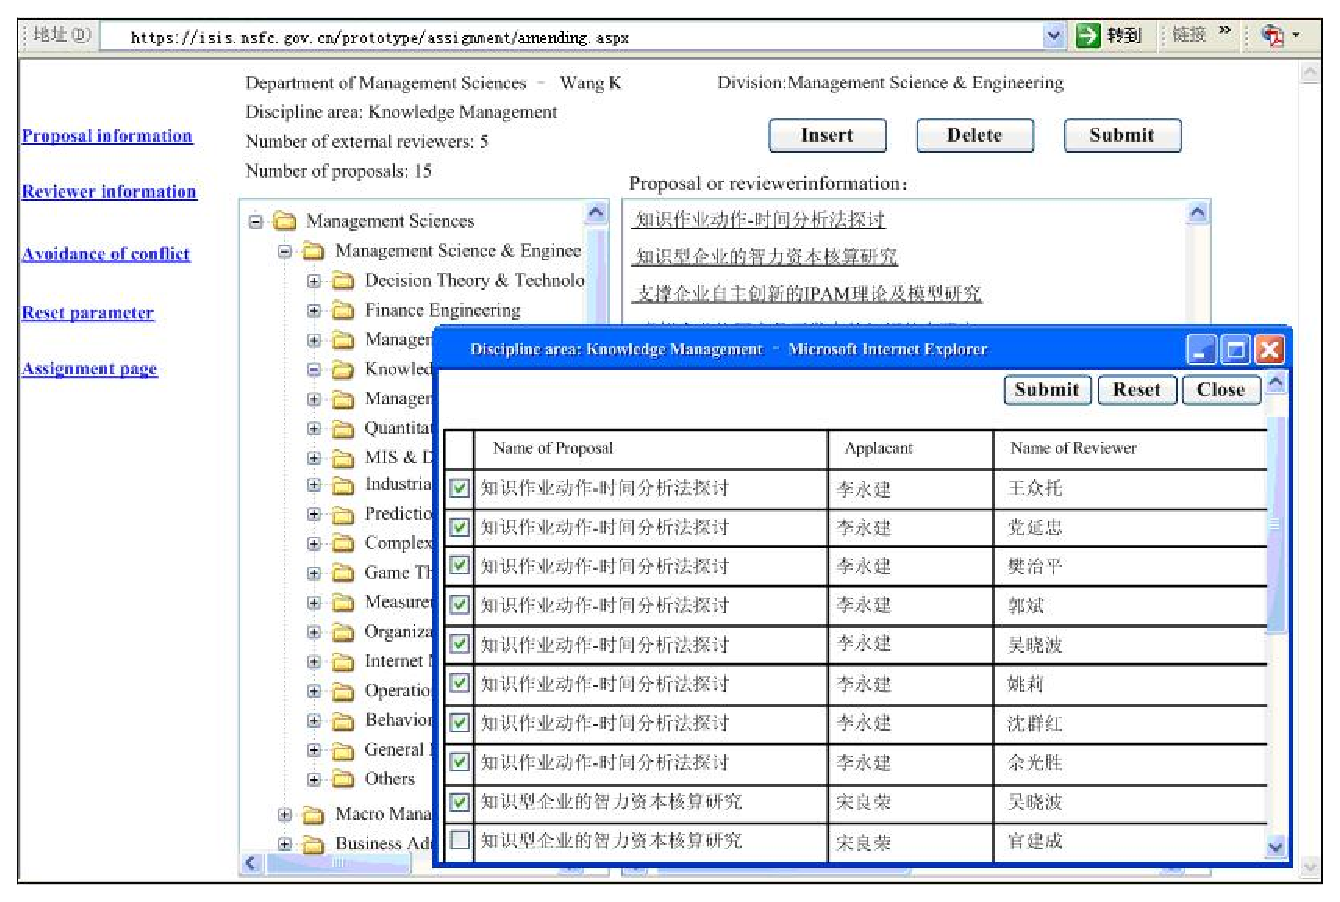
\includegraphics{10}}
  \caption{The relationship between the  clustering coefficient  and
    the scale ratio}
  \label{fig:cc-ration}
\end{figure}

With the increase of $W$, the clustering coefficient does not
decrease, but increases slightly. Although the data is not very ideal,
they are consistent with the objective network. On the one hand, the
scale ratio $W$ is not continuous, but just discrete points; on the
other hand, according to the studying on the clustering coefficient in
section 3, thre fluctuation is small. Such insignificant positive correlation between the clustering coefficient and the scale ratio illustrates the balanced growth between Wikipedia user nodes and the topic nodes, which is essential for the steady change of the clustering coefficient. 


\section{Conclusion}
\label{sec:5concl-disc-}

Analysing the interaction between users and topics is important to
understand the mechanism of content collaboration behavior. 
In this paper, we propose a knowledge collaboration network model
using  Wikipedia archive data, and analyze the statistical
properties of the network. We have found that the one-dimensional network of this model is a scale-free structure and its distribution function is subject to the characteristics of the power law, BA scale-free structure growth and preferential attachment. From the observation on the changes of the average degree, the number of the relationships in the knowledge collaboration network shows cyclical fluctuations, and the links tend to closer. In the one-dimensional knowledge collaboration network, with the increasing of network size, the clustering coefficient will be inclined to a non-zero constant(0.65). Meanwhile, the network average distance is less than 4, which reflects that the small-world effect exists obviously in the knowledge collaboration network. At the early stage of the network development, the network doesn’t possess hierarchical topology. However, when the network size increases with time, the network gradually reveals certain level of hierarchy. In addition, in the knowledge collaboration bipartite network, the theme distribution of the subject node is the same as the degree distribution of BA model of the one-dimensional network: subject to the power-law distribution and possessing the characteristic of “long tail”. In the one-dimensional network, the network density grows with the growing of the scale ratio, however, the clustering coefficient increases concussively, which presents an insignificant positive correlation between the clustering coefficient and the scale ratio. The limitation of this study is root from the
limited data processing ability to the
huge Wikipedia data. We have to select some slice the data and divided
into sub-networks. The
phrase change of hierachicl topology is  not included in this paper
neither. All will be the future research works.  


\section*{Acknowledgment}
\label{sec:acknowledgment}
This work was partly supported by the National Natural Science Foundation of China (NSFC, Project No. 70871006).


\bibliographystyle{elsarticle-num}
\bibliography{../../bibtex/elsevier,../../bibtex/emerald,../../bibtex/chinese,../../bibtex/jstor,../../bibtex/citeseer,../../bibtex/acm,../../bibtex/wiley,../../bibtex/book,../../bibtex/thesis,../../bibtex/ebsco,../../bibtex/old,../../bibtex/ieee,../../bibtex/internet,../../bibtex/ssrn,../../bibtex/apa,../../bibtex/blackwell,../../bibtex/sage,../../bibtex/springer,../../bibtex/MESharp,../../bibtex/taylor,../../bibtex/arXiv}
\end{document}
